
\documentclass[12pt]{article}
\title{ECE 141 Homework 4}
\usepackage{subcaption}
\author{Lawrence Liu}
\usepackage{graphicx}
\usepackage{amsmath}
\usepackage{placeins}
\newcommand{\Laplace}{\mathscr{L}}
\setlength{\parskip}{\baselineskip}%
\setlength{\parindent}{0pt}%
\usepackage{xcolor}
\usepackage{listings}
\definecolor{backcolour}{rgb}{0.95,0.95,0.92}
\usepackage{amssymb}
\lstdefinestyle{mystyle}{
    backgroundcolor=\color{backcolour}}
\lstset{style=mystyle}

\begin{document}
\maketitle
\subsection*{Problem 5.9}
The transfer function is $$\frac{Y}{R}=\frac{5}{(s(s+2)+5+5\alpha s)}$$, therefore the characteristic equation is $s(s+2)+5+5\alpha s=0$, therefore we have $b(s)=5s$ and $a(s)=s^2+2s+1$
Therefore we have that $L(s)=\frac{5s}{s^2+2s+1}$, therefore 1 line will approach asymptotes centered at $-2$ and leaving at angles $180^{\circ}$. Furthermore, the departure angle from the poles
$-1\pm 2j$ is $\mp153.4^{\circ}$ and the arival angle to the zero at 0 is $180^{\circ}$, therefore the root locuses are at 
\\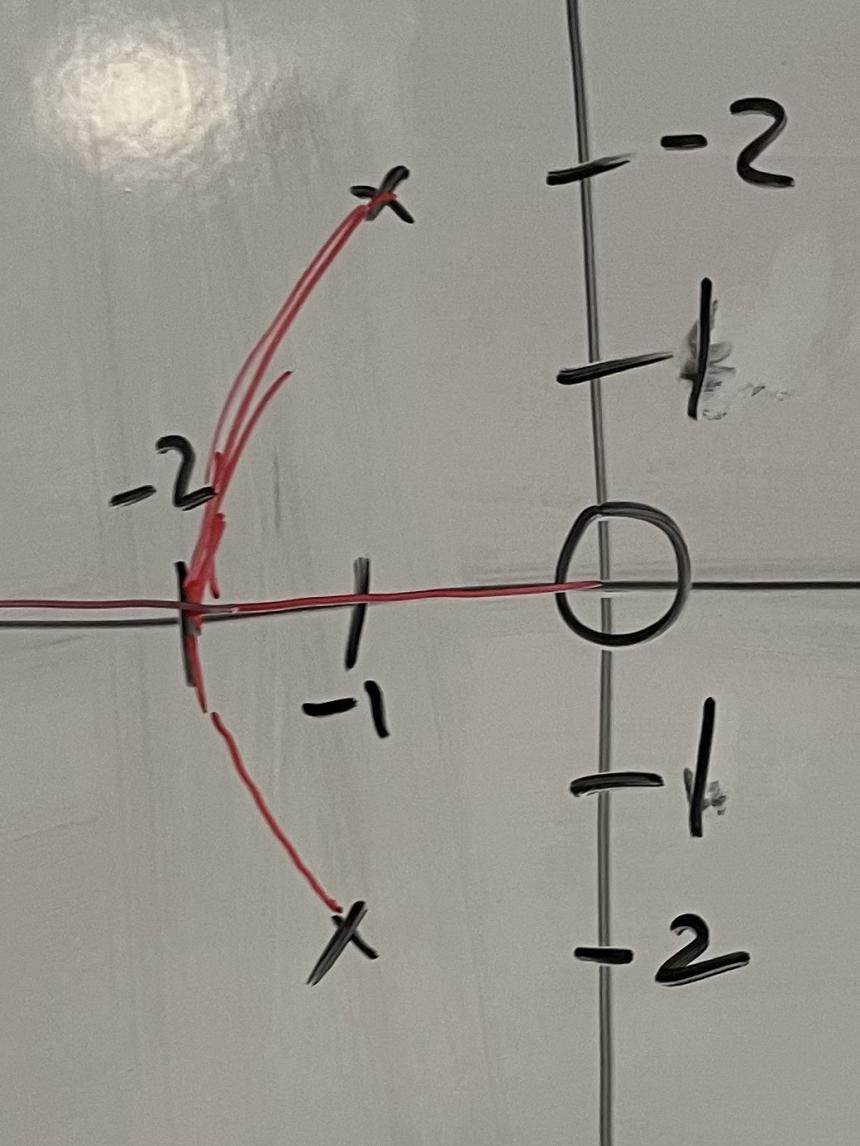
\includegraphics[scale=0.25]{Problem1fig1.jpg}\\
When $\alpha=0$, there are poles at $-1\pm 2j$, when $\alpha=0.5$, there are poles at $-2$ and $-2.5$, and when $\alpha=2$, there are poles at $-0.432$ and $-11.568$, therefore the plot of the poles looks like
\\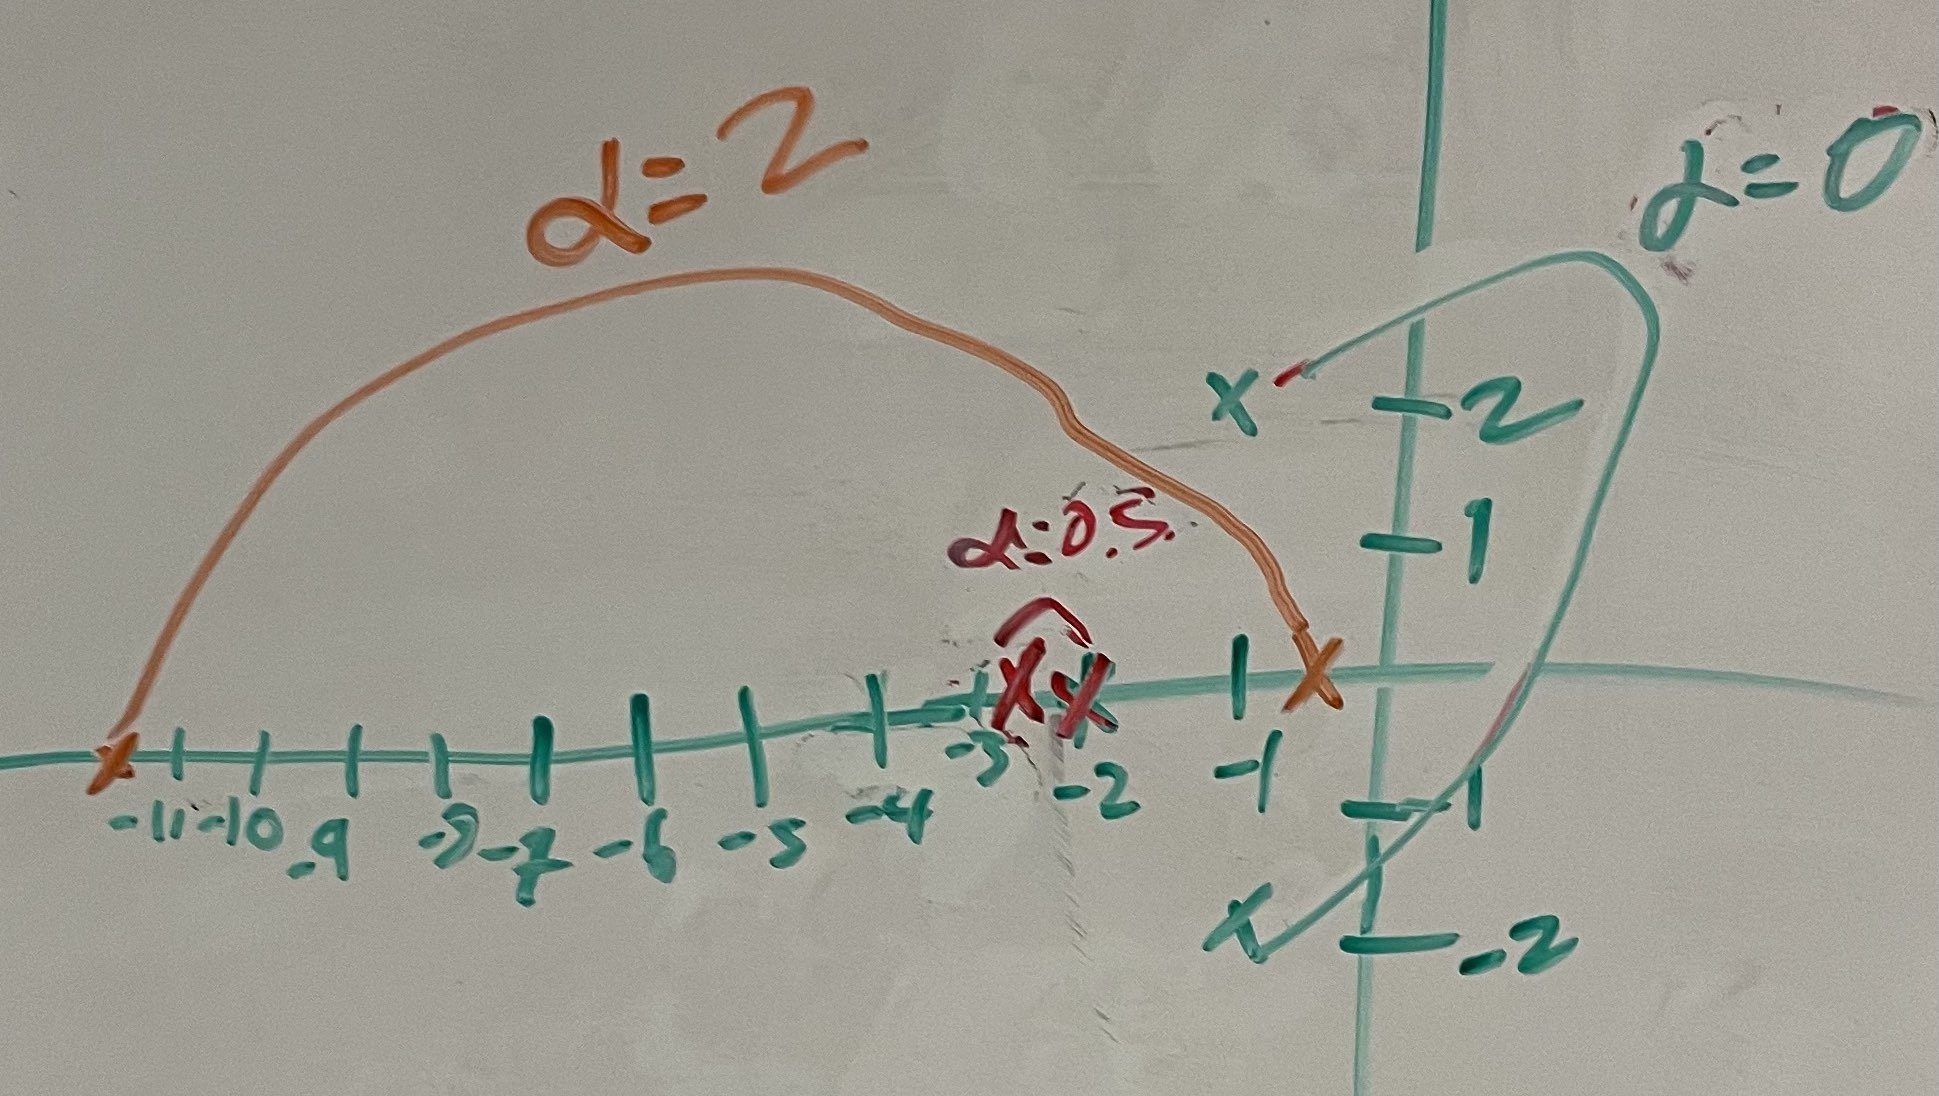
\includegraphics[scale=0.15]{Problem1fig2.jpg}\\
Therefore since $alpha=0$ the step response will be underdamped since it has poles with imaginary components, and for $\alpha=0.5$ the damping factor $\zeta=\frac{4.5}{2\sqrt{5}}$ and when 
$\alpha=2$ the damping factor $\zeta=\frac{6}{\sqrt{5}}$, therefore the plot of the step responses would look like
\\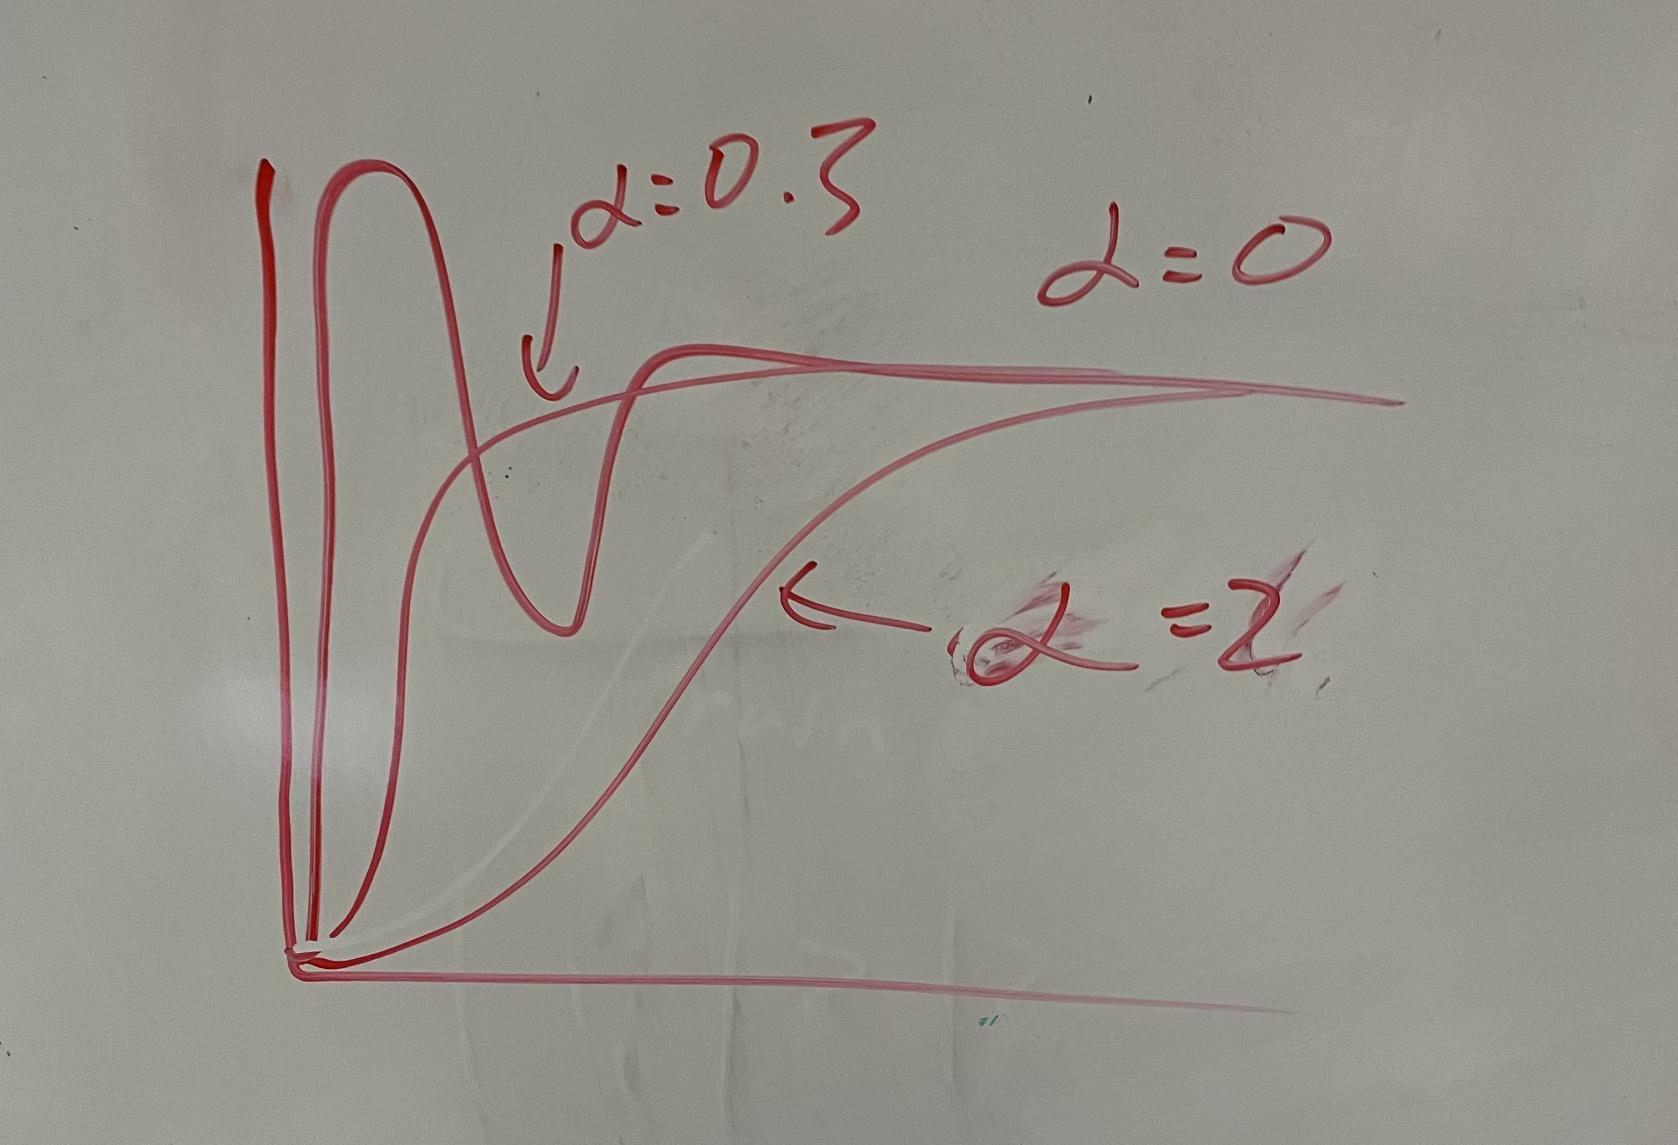
\includegraphics[scale=0.15]{Problem1fig3.jpg}\\
With the following matlab code we can verify it
\begin{verbatim}
sys = tf([5],[1 2 5]);
step(sys)
stepinfo(sys)
hold on;

sys = tf([5],[1 2+2.5 5]);
step(sys)
stepinfo(sys)

sys = tf([5],[1 12 5]);
step(sys)
stepinfo(sys)

hold off;
legend('alpha=0','alpha=0.5','alpha=2')
\end{verbatim}
Which produces the following plot.\\
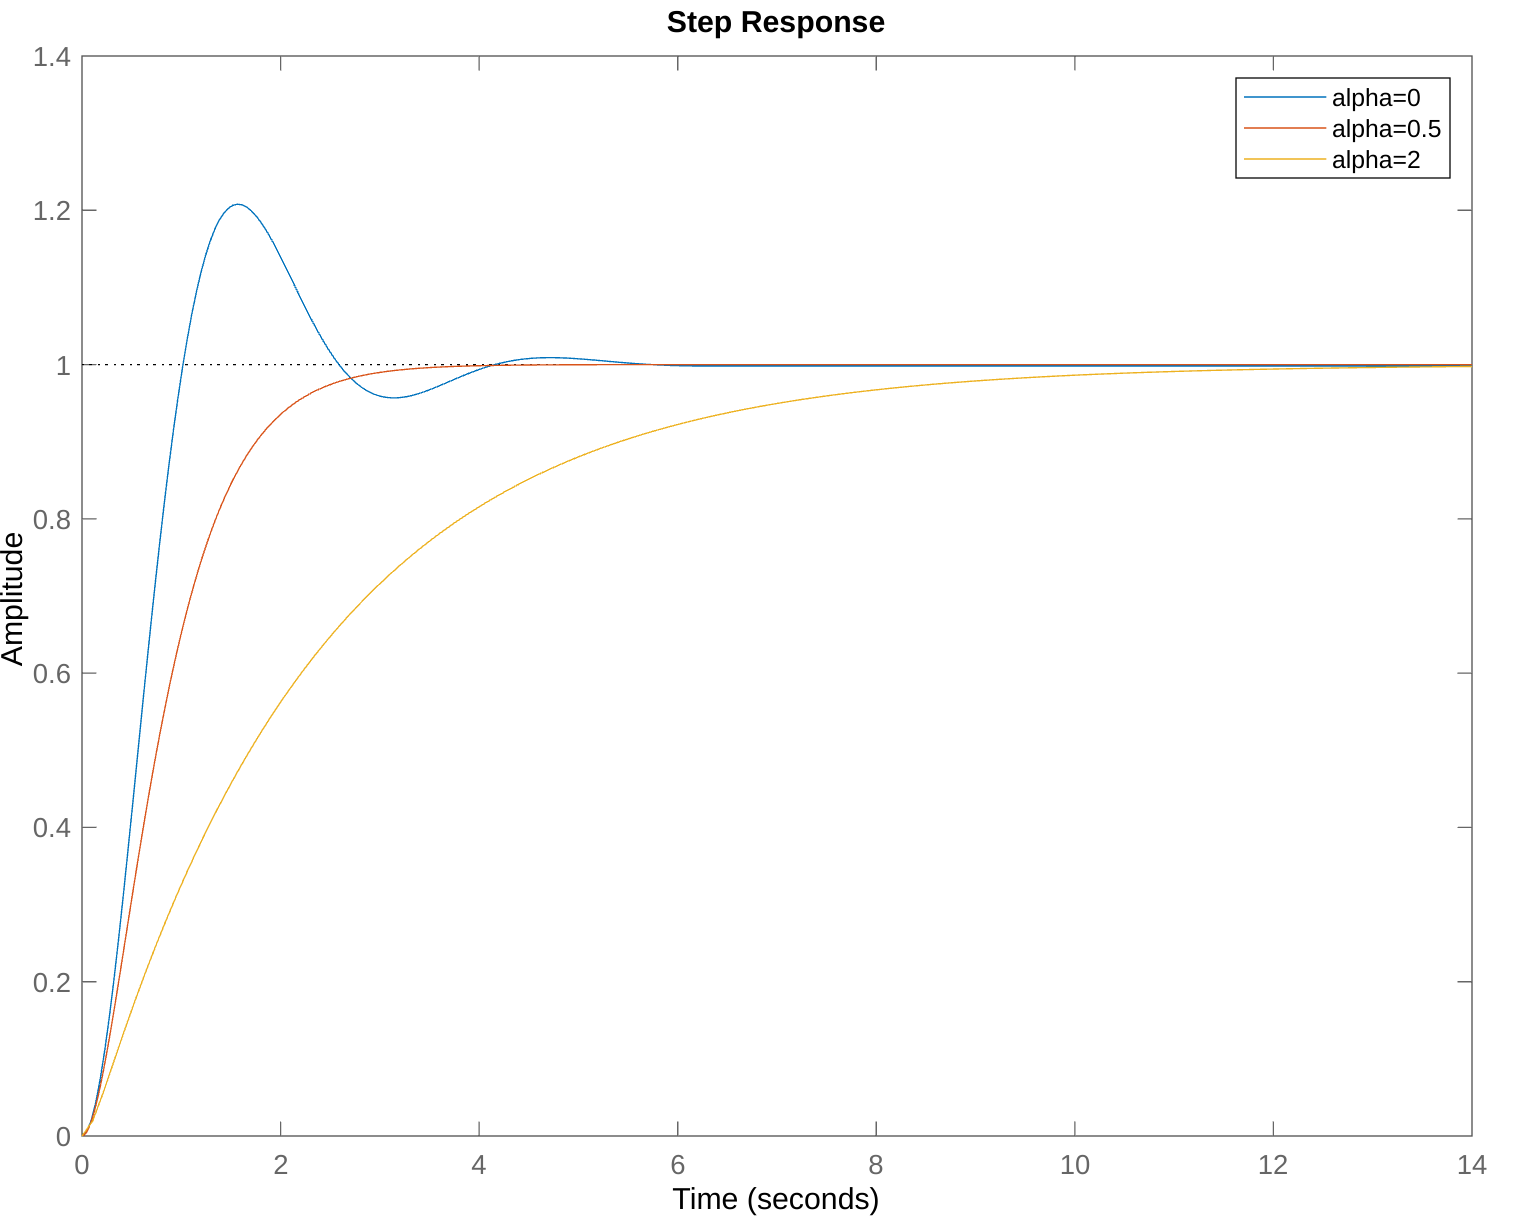
\includegraphics[scale=0.25]{Problem1fig4.png}\\
\section*{Problem 5.13}
\subsection*{(a)}

\end{document}